\chapter{Background}
The most challenging part of this work has been dealing with low-cost sensors. These products are considered really interesting from different points of view, from the power consumption to the easiness of integration in PCBs, but at the same time some effort is required in order to get the most out from them. This is the subject of different studies, some of them focused on the performance/energy trade-off of the Bluetooth Low Energy standard, while others are trying to implement different mechanisms of time synchronization that could work between different sensors. Another field of exploration is the so-called sensor fusion: in these studies, more low-cost sensors are used in parallel, to join all their values and finally get more precise results by using adequate algorithms. In this background section, the goal is to sum up some of the most relevant studies and experiments that have been conducted on these fields, while exploring some state-of-the-art solutions that are available on the market. 

\section{Bluetooth Low Energy: standard overview and throughput analysis}
The choice of radios and communication protocol is always a hard one when dealing with sensor networks. As different technologies offer different performances in different areas, the choice should be coherent with the kind of data we are dealing with. For example, some aspects that should be considered are throughput, latency, number of nodes and compatibility: while the first two could be critical in healthcare applications, compatibility could be crucial when dealing with sensor devices aimed at the mass market. In particular, the Bluetooth 4.0 standard (also called  Bluetooth Low Energy) aims at maximizing device connectivity and energy efficiency, with the drawback of a limited throughput.

\paragraph{The Bluetooth Application Layer.} When dealing with BLE chips, usually the final user can have control on the Application Layer of the communication protocol, while lower levels (Host and Controller) usually can't be optimized by the developer. In particular, the top level is composed of:
\begin{itemize}
    \item Logical Link Control and Adaptation Protocol (L2CAP), takes care of protocol/channel multiplexing with error and flow control
    \item Security Manager, responsible for device pairing and key exchange
    \item Attribute Protocol, allows the device to expose a set of attributes and relative values
    \item Generic Attribute Profile (GATT), defines a way to interact with those attributes: devices can be clients or servers. 
    \item Generic Access Profile (GAP), regulates the procedures of discovery and connection with other devices.
\end{itemize}
\paragraph{Data Exchange.}When the connection completes, a device will assume the role of the GATT client, while the other one would be the GATT server. This means that data exchange happens only at the GATT level: the server will expose a number of \textit{characteristics}, each one being an array of bytes (with the maximum set to 512 B), grouped into \textit{services}. The GATT client can interact with those characteristics, depending on the \textit{properties} of each one. Those properties can be:
\begin{itemize}
    \item \textbf{Read}: the client explicitly requires the value of the characteristic, the server answers accordingly
    \item \textbf{Write}: the client writes the value of the characteristic
    \item \textbf{Notify/Indicate}: the server will inform the client of a new value of the characteristic, without the need of an explicit request. Indications also include an application level acknowledgement of the notification. 
\end{itemize}
Usually notifications are preferred, as only one packet should be exchanged for each new value: no request and no acknowledgment are necessary. 

A particular characteristic of the BLE protocol is the usage of the so-called Connection Events (CE). Data exchange can only happen during these events, and between them the radio goes to sleep: this duty cycled behaviour is one of the reasons of the low energy consumption of the standard. The time interval between two consecutive CEs is called Connection Interval (CI), with allowed values going from 7.5~ms to 4~s (at 1.25~ms steps). These parameters are negotiated at the connection setup, but they can be changed at any time during the connection. 

\paragraph{BLE Throughput.}  The standard defines the data transfer rate to be 1~Mbit/s, but the effective value depends on link quality, layer overheads and hardware constraints. Some studies tried to calculate it, obtaining different results:
\begin{itemize}
    \item Gomez (2011) \cite{gomez2011modeling} reports a maximum throughput of 236.7~kbit/s, by representing the connection through an analytical model. The main flaw of this approach is that it does not take into consideration the hardware constraints of low-cost BLE nodes. 
    \item In \cite{mikhaylov2013performance}, performances of Bluetooth Low Energy are compared to other wireless solutions, reporting a link layer throughput of 122.6~kbit/s: this value is not considering upper layers of the standard, hence it is not considering the packet overhead coming from the application layer.
    \item In \cite{gomez2012overview} presents an overview on the standard, carrying out a practical experiment on throughput: two CC2540 devices, from Texas Instruments, are configured to send data at the maximum possible speed, with Connection Interval set to the minimum possible value. The resulting throughput is 58.48~kbit/s.
    \item \cite{giovanelli2015bluetooth} is probably the most extensive one, as multiple BLE modules are used, each one with its own stack and firmware. It underlines the importance of Connection Intervals in maximizing the throughput. To sum up, the study concluded that the maximum application level throughput that can be achieved is 64~kbit/s, by fine tuning the values of CIs and by using buffer-like structures to maximize the data to send out at each Connection Event.  
\end{itemize}

\section{Bluetooth performances in Sensor Networks} 
After understanding how BLE works and how to get the most out of it when dealing with a single node, I focused on more complex configurations. In \cite{reich2020bluetooth}, the goal is to set up a sensor network and to find the highest possible data rate, in order to use data coming from IMU devices for Human Activity Recognition (HAR) purposes. The researchers state that, for a good HAR analysis, they would require data coming from as many sensors as possible, with a sampling data rate between 25~ms (40~Hz) and 35~ms (28~Hz).     

From the technical point of view, they decided to use notifications to reduce the number of exchanged packets to the bare minimum, left the original setting of the sensor node with regards to the Connection Interval and used a Python script to harvest all the data and perform the analysis on them. To make the performance analysis as complete as possible, they had 20 sensor nodes available, and used different computers as clients, each one with a different Bluetooth adapter. To be more precise, they used up to 20 \textit{Arduino Nano 33 BLE Sense}, with 9-axis IMU, barometer and temperature sensors connected at different computers, each one with its own Bluetooth Adapter. 

The main test consisted of finding the maximum number of Bluetooth sensors that can be connected to a single client, varying the data rate between 25~ms and 35~ms and trying all the different computers. The results then were compared considering the percentage of lost packets. The results table in the paper makes it evident that the choice of the Bluetooth adapter is quite important: 10 sensors connected, with data rate of 35ms, resulted in 20\% data loss for the Macbook Pro 2014, while the Intel NUC 8 shows a loss percentage of 0.07\% only. 

To sum up this experimental analysis and its conclusions:
\begin{itemize}
    \item Reseachers showed that the best performance are obtained by using a DeLock Bluetooth Adapter, based on the Broadcom BCM20702A0 chip. It managed 13 simultaneous connections, with a loss percentage of 0.03\% with the sensors set at 35ms data rate.
    \item Notifications perform better than indications in high performance sensor settings.
    \item There are big differences in performance between Bluetooth modules.
\end{itemize}
\section{An example of time synchronization from National Instruments}

National Instruments is a company that produces test equipment and virtual instrumentation software. One of the most important application for their products is data acquisition, and  they are considered one of the leaders thanks to their experience in this field. 

An article from their website \cite{NISync} states that data should be appropriately synchronized in time to be accurately analyzed, and they propose a list of approaches to fulfill such goal using their products. In particular, they focus on their PXI platform.

\paragraph{The PXI Platform} PXI is defined by National Instruments as the standard for automated test and measurements. It is a family of modular instruments and I/O elements that can work together, with specialized synchronization algorithms and software. The main core of the system is the chassis with its own controller, that accepts a certain number of measurement modules and provides the same functionalities to all of them. 

In the latest version of the platform, called \textit{PXI Express}, developers included different elements thought for precise time synchronization:
\begin{itemize}
    \item A 10~MHz backplane clock, offered in parallel by the chassis to all connected component
    \item A single-ended trigger bus
    \item A star trigger signal, accurately developed such that the connection to all the modules have the same length
    \item 100 MHz differential clock and differential triggers, with increased noise immunity. 
\end{itemize}
The user can then freely choose the way to share clock and trigger signals between all modules. Every option has its own advantages and disadvantages considering signal skew, signal integrity, compatibility with external modules and necessity for external controllers.
For example, the 100~MHz clock provides a skew that is less than 250~ps, while the star trigger signal performs a skew that is less than 500~ps. Both of them provide the best signal integrity between all the solutions. 
Of course, the listed solutions are intended for modules connected to the same chassis, but some components can perform synchronization between different ones by using GPS or IRIG-B standards.  

\paragraph{Synchronization Techniques} In order to effectively perform time synchronization, National Instruments defines the differences between two types of devices:
\begin{itemize}
    \item Sample Clock Timed Devices. These devices use a \textit{sample clock} that controls when the samples are acquired. For example, SAR ADC converters usually have a dedicated convert line that, when toggled, triggers an immediate conversion.
    \item Oversample Clock Timed Devices. In this case, the device requires a free-running oversample clock that drives the conversion while keeping the ADC operating: the resulting samples are generated at a rate that is a division of the original clock. These devices can't be controlled by external signals, hence synchronization is more complicated.
\end{itemize}

To synchronize the sample clock, different options are possible:
\begin{itemize}
    \item Share sample clock directly. A master device will share its sample clock to the slave ones, using one or more of the backplane of the PXI chassis.
    \item Derive the sample clock from a common reference clock. The 100~MHz differential clock is divided to generate the sample clock, distributed to all the devices. A dedicated software from NI is able to perform all the necessary configuration for the user.
    \item Share the trigger signal. This is the simplest but the loosest synchronization mechanism, as all the devices will only receive the same trigger signal. In this case, usually devices drift in time, as sample clocks are not locked together. 
\end{itemize}

When dealing with oversample clock timed devices, the only possibility is the reference clock synchronization. First of all, the ADCs on the devices are reset and configured to generate samples after the same number of clock cycles. Then, the acquisition is started synchronously with a shared trigger signal. During the reset and sampling procedures, all the devices are locked to the 100~MHz clock signal provided by the PXI chassis. 

\paragraph{Conclusions} National Instruments solutions are, of course, the best synchronization mechanisms that I found during the research, offering extremely high performances and a great software support for easy configuration. All of this comes at certain costs: 
\begin{itemize}
    \item All the modules should be physically connected to the chassis, and no wireless connection is possible (it wouldn't support this kind of synchronization)
    \item The modules should support the National Instruments standard. Even if it is open and can be implemented by manufacturers quite easily, it is targeted at high-cost, high-precision measurement tools.
    \item The PXI system is extremely expensive: the cheapest controller has a cost that is around 1400€ (PXIe-1090), with no module installed. 
\end{itemize} 
\section{Precise Sensor Synchronization in Robotic Computing}
Paper \cite{liu2021brief} summarizes the development of time synchronization systems done by a development team interested in different commercial robotic and autonomous driving products. They underline the importance of time synchronization by presenting the example of a camera and a Laser Imaging Detection and Ranging (LiDAR) sensor: if the measurements are not aligned on time, those would cause inaccurate and ambiguous view of the environment, with the possibility of catastrophic outcomes.

\paragraph{Addressed issues and goals} The main goal of the researchers has been to \textit{ensure that sensor samples that have the same timestamps correspond to the same event}. To reach this objective, they developed two kinds of synchronization: intra-machine (synchronizing sensors within a particular machine) and inter-machine (synchronizing sensors across different machines). They reported some examples to motivate the need for synchronization:
\begin{itemize}
    \item Perception tasks: in order to fuse 2D information from cameras and 3D information from LiDARs, their data must be synchronized (intra-machine).
    \item Localization tasks: autonomous machines use multi-sensor fusion algorithms to obtain accurate localization estimations, for example fusion of camera and IMU information (intra-machine). It was observed that a misalignment of 40~ms can cause a 10~m translational error with a 3° rotational error.
    \item Interaction with other machines: when dealing with robots (or other devices) collaborating together, their synchronization could be critical (inter-machine). The example of two Road Side Units is reported: they use the position of a vehicle with the corresponding timestamp when calculating its speed. If the timestamps are not coherent, the speed may vary significantly.      
\end{itemize}

\paragraph{Synchronization principles} In order to perform the synchronization, two requirements have been found: first, all sensors should be triggered simultaneously, and secondly, each sensor sample should be associated with a precise timestamp. This is challenging, as all sensor have different triggering and time-stamping mechanisms. 
Four (theoretical) principles have been found:
\begin{itemize}
    \item Externally-triggered sensors should be triggered in hardware. Camera and IMUs can be easily triggered via software, but the driver stack may generate different latencies that can't be precisely predicted. The solution is the trigger through custom hardware.
    \item Use a shared timer to simultaneously initiate internally-triggered and externally-triggered sensors. Internally-triggered sensors, such as LiDARs, usually accept an external initialization signal, then they would generate samples at a defined rate. It is important to use a common timer to generate both this initialization signal for them and the trigger signal for the other devices.  
    \item Synchronize machine timer with GPS global clock. If inter-machine synchronization is necessary, it is important that their time sources are aligned to a global high-precision atomic clock, like the time data transmitted by GPS satellites.
    \item Obtain the timestamp for a sensor sample as close to the sensor source as possible. Again, the easiest way would be to timestamp samples via software, but as explained before this can be not so precise. A better solution is to obtain the time information directly at the sensor interface, that is, when the sensor data is received by the SoC from the off-chip sensor. 
\end{itemize}

\paragraph{Adopted Solution} The researchers decided to adopt an FPGA-based solution to satisfy all the principles stated above. In particular, the Xilinx Zynq Board contains a general-purpose ARM CPU to run the software components, with a lot of I/O interfaces for all the connectivity necessities.

A serial port interface accepts GPS global data, distributing it to all hardware and software timers. Trigger and timers units, designed in hardware, manage the triggering and the initialization of the sensors. Finally, Serial port, CAN and MIPI interfaces are designed to automatically assign timestamps to the samples as soon as they're received from (respectively) the IMU, camera and radar sensors. 

The obtained circuit is lightweight (6.9K LUTs and 7.1K Registers). Accuracy is particularly good, as timestamping is performed at cycle-level precision for most sensors, while the LiDAR sensor (internally triggered) showed variations within 100~\(\mu\)s.

\section{Synchronization in Wireless Sensor Networks: Review}
Paper \cite{djenouri2014synchronization} reviews synchronization mechanisms aimed at Wireless Sensor Networks, in which the single low-cost, low-power nodes should perform synchronization and transmission by themselves. It also underlines the importance of correlation between different reports from different devices to perform data fusion, time-division multiple-access scheduling and to use real-time applications, even if the delay variability of the wireless connection and the computation limitations of the nodes make the issue even more complex. 

\paragraph{General Concepts} The main idea regarding synchronization in this paper is to mathematically estimate the oscillators in each node, and then implement some sort of message exchange mechanism between them. The goal is to model the differences between the clocks in the devices and modify their behaviour accordingly.

The \textbf{clock models} analyzed, on which the synchronization algorithms will base their estimations, are:
\begin{itemize}
    \item Offset-only model. The local clock of a node is defined as in \ref{offset-only} 
    \begin{equation} \label{offset-only}
        C_i = t + \theta_i 
    \end{equation}
    where \(t\) is an ideal clock and \(\theta_i\) the offset relative to that ideal clock.
    \item Joint skew-offset model. This provides long-term estimators, at the cost of augmented calculation complexity. The local clock can be approximated as done in Equation \ref{skew-offset}
    \begin{equation} \label{skew-offset}
        C_i = \alpha_it + \beta_i 
    \end{equation} 
    where \(\alpha\) is the absolute skew and \(\beta\) is the offset of the node clock. 
\end{itemize}

Once the clock model has been defined, the \textbf{message exchange mechanism} should be chosen:
\begin{itemize}
    \item Sender to Receiver: nodes periodically exchange timestamped synchronization messages. This happens in 4 steps. Node \(n_1\) sends a packet with timestamp \(t_1\). The second node \(n_2\) receives it, with timestamp \(t_2\), and replies with timestamp \(t_3\). At the end, \(n_1\) timestamps the reception of the reply with \(t_4\).
    \item Receiver to Receiver: in this case, a reference (defined exploiting the property of the physical broadcast medium) is used to broadcast messages simultaneously to all devices, that will timestamp the reception event as \(t_1\) and \(t_2\). Those samples are the only ones used for synchronization purposes. 
\end{itemize}

Timestamps obtained through these mechanisms are not totally accurate, as the messages go through a path that may vary nondeterministically to different factors: send time (packet generation and transmission time), medium access time (MAC level), propagation time, reception time (packet processing). The receiver to receiver method removes send and access time from this path.

Once the method has been defined, the paper reports three kind of synchronization categories: 1) event ordering, which is the simplest form, 2) synchronization to a reference and 3) relative clocks. The last one is the most used in the analyzed algorithms, and it consists in maintaining inside the node the information about relative skew and offset to other nodes. 

\paragraph{Main issues} The paper proceeds with a list of all the possible problems in maintaining a good time synchronization between the nodes:
\begin{itemize}
    \item Fast drifting. This is considered the main issue, and it derives from the usage of cheap circuitry components (in particular, oscillators). Usually sensor nodes present two kind of oscillator, a high-speed one (usually with high drifting), and a lower speed one, used in energy-saving situations, that is usually more precise but provides less granularity. 

    Of course, a fast drifting clock requires frequent re-synchronizations, that may result very expensive. 
    \item Node limitation. If the synchronization requires some calculation at the node level, usually the calculation power at disposal is very low, and all of it should be optimized as more as possible. For example, some nodes may not dispose of FPU units, and FP calculation may be implemented at software level, causing delays.
    \item Delay Variation. This is intrinsic to the message exchange mechanism, as there is some nondeterminism when considering message delays. Usually, this issue can be overcome by timestamping packets at the MAC layer, but this solution is both not portable between different devices/protocols, and not applicable to devices whose software stack hides the lower level to the developer.
    \item Fault Tolerance. These synchronization mechanism neglect aspects like nodes failure or packet losses, and provide no recovery algorithm in those cases.
    \item Accuracy measurements. The accuracy of such protocols is extremely difficult to assess, as instantaneous local times from the nodes should be captured at the same physical time. 
    \item Impact of empirical parameters. All the possible implementations relay on some parameters regarding the message exchange, in particular, the number of rounds before estimation \(k\) and the period between rounds \(T\). 
    
\end{itemize}

\paragraph{Conclusions}
The main issue found in this paper with regards to time synchronization is, without doubts, the clock drifting issue. Two solutions have been found: frequent message exchange in the simpler offset-only clock model, or less messages using the more computationally expensive skew-offset model. The choice of the final model is up to the developer, that should choose the least expensive of the two considering the node and the connection protocol at their disposal.

The second big challenge is the delay of message exchange/handling. The usage of the Receiver to Receiver model will reduce that delay, but optimizations can be performed using a MAC-layer timestamping solution (when possible).  
\section{Bluesync: a Time Synchronization protocol for BLE}
Paper \cite{asgarian2021bluesync} explains an interesting protocol that can be used for time synchronization purposes when dealing with Bluetooth Low Energy devices, like sensor network nodes. The article stresses the importance of a low-cost and high-efficiency mechanism that can work on these resource-constrained IoT nodes.  

In particular, BlueSync is defined as a synchronization service for BLE beacon devices. BLE Beaconing is an advertising mode, supported by Bluetooth Low Energy, that enables the exchange of data between devices without the need of entering a bonded connection: the server device will \textit{advertise} its data, while the client can read it doing a \textit{scanning} operation. This protocol does not present any time synchronization service. 
BlueSync makes the system work in two different stages: first, there is a timeslot (few seconds) in which synchronization packages are exchanged, then, the second timeslot will allow the execution of synchronous tasks. Of course, the time interval between the two stages should be decided with care, as precision will depend on that. The developers showed that the node can proceed with 10 minutes of synchronous tasks without the need of re-synchronization, still with a good time precision. 

The devices tested in the work are from Nordic Semiconductor, in particular an nRF51 (16~MHz ARM Cortex-M0) and an nRF52 (64~MHz ARM Cortex-M4).

\paragraph{Implementation} The implementation of the BlueSync protocol is presented in three steps, that are reported and explained as follows.
\begin{itemize}
    \item Timestamping. The main problem encountered when dealing with BLE beacons is that they usually exchange data in three different channels, with non-predictable delays. With proper modifications of the registers of the Nordic devices, the developers managed to set the transmission (advertising) and the reception (scanning) of the data on a single channel, both on the server and the client devices. Once this has been resolved, the problem of delays is addressed and solved by precisely deciding the moment at which packets are timestamped. Also in this case, a particular function available on Nordic devices has been used: PPI, Programmable Peripheral Interconnect. It allows the execution of a particular task at the end of a transmission event in a very precise manner, generating a standard deviation in timestamping of less than 50~ns. Of course, the timestamps collected after the radio event are sent in the next packet, hence the synchronization stage requires more than one packet to be transmitted (to retrieve all the necessary timestamps).
    \item Frequency Drift Estimation. As soon as all synchronization packets have been received, the contained timestamps are used to estimate the offset and the drift of the nodes clocks. This is a calculation that is performed on the node itself, and should be optimized due to their hardware constraints and available functionalities (for example, the Floating Point Unit could be missing). Researchers tried two different algorithms: Linear Regression and Average Error. Both have been tested with either 8 or 16 timestamps, sent at regular intervals, with the latest packet initiating the execution of the synchronous task. The two algorithms show different performances on the two different processors, due to the different architectures: when dealing with heterogeneous hardware, it is important to fine-tune the choice of the algorithm. 
    \item Tick Adjustment. The last part of the mechanism consists in applying the estimation calculated before to the number of ticks necessary to reach the next point in time to execute the synchronous task: the floating-point result should be converted to an integer and then set as timer interrupt. These adjustment require clock cycles, and their impact should be taken into consideration, for example recalculating the ticks every 100 runs.
\end{itemize}

\paragraph{Conclusions} To sum it up, BlueSync is a synchronization protocol aimed at BLE Sensor Networks, compatible with commercial SoCs. Its implementation consists mainly in improving timestamping of BLE packets and choosing the most optimized frequency-drift estimation algorithm. The resulting timing accuracies, in the tests performed in the laboratory, are around 320~ns for 60~s. They assure that the system can provide good accuracy with synchronization timeslots every 10 minutes, with synchronization windows of less than 2 seconds. Even if these results are particularly good, it is important to notice that they are possible only with the functionalities available on the particular Nordic devices used, hence they may not be applicable to other SoCs on the market. 
\section{An application example: IMU-Enabled Posture Monitor}

Paper \cite{petropoulos2020wearable} reports an interesting application for synchronized sensor nodes that is worth analyzing in this thesis: a monitoring system for sitting posture that uses wireless motion sensors attached to the user's back. Different sensors are used, and data coming from them is then fused together.

\paragraph{Implementation} The article focuses on three main points:
\begin{itemize}
    \item \textbf{Data Sensing} The required hardware needs to be small, comfortable to the user and compatible with all his possible movements. Of course, it needs to be powered via rechargeable batteries. All these requirements are the typical ones of IoT applications, and are supported by the new MEMS-based IMUs: small, low-power devices that provide all the necessary information.

    In this application, 6-degrees of freedom IMU sensors (namely, accelerometer and gyroscope) are installed on two prototypes modules that are attached to the upper and lower back of the user, parallel to their spine. The stream of these devices will then be used and elaborated to provide the spine misalignment devised into a pair of angles. Starting from this data, the system is capable of detecting spine inclination and lumbar placement in all the four directions. 

    Two main problems in using IMUs in this application have been assessed: first of all, the low-resolution, noise-corrupted and biased signals coming from these kind of sensors require a quite heavy processing stage to get quality data. Secondly, as it is only possible to detect angle changes when using accelerometer and gyroscope sensors, a calibration phase (with the user collaboration) is necessary before starting to harvest posture data.

    \item \textbf{Data Transmission} In this application, Bluetooth Low Energy has been considered the best solution. It has been increasingly used in wearable applications, it offers power-efficient operation and, mostly important, it is natively compatible with a lot of devices that could work as data aggregator, like smartphones.

    \item \textbf{Data Processing} As stated before, data coming from these IMU sensors requires some sort of refining to clean the signal and get the interesting angle information. Raw data is processed by means of a weighted moving average filter, then an Explicit Complementary Filter (ECF) algorithm is used to fuse all the information together and extract the two angles. All of this is performed on the smartphone of the user, that provides the required calculation capabilities (not available on the sensor nodes). 
\end{itemize}

\paragraph{User Interface} In order to use the posture monitor system, the user will first participate in a placement and calibration phase. Once it's done, the monitoring session starts, and the user is notified via vibration every time the angle threshold indicating a bad posture are violated. Once the session is complete, the user can analyze on the smartphone their posture behaviour, while the data is uploaded to a cloud-based application that can monitor the posture over time, maybe using Artificial Intelligence algorithms. 

\paragraph{Evaluation} To perform evaluation of the entire system, the two sensor boards have been attached on Pan/Tilt units. Then, different pre-defined couple of angles are simulated by the servo motors of the units, and then compared by the ones estimated by the IMUs. Repeated tests showed that the system is very reliable, showing errors that are distributed in a Gaussian shape and that are less than 0.1 degrees. The paper explains that observed errors are caused by the intrinsic error noise, and that the IMU calibration procedure is very useful to reduce biases, misalignment and gain errors. 

\paragraph{Conclusions} The article showed how data coming from low-cost sensor nodes, with limited computational capabilities and restrictive power constraint, can be quite precise when dealing with medical applications. Of course, there is the need of extensive post-processing work, usually performed by algorithms that run on more powerful devices, but the result is an user-friendly application that can be used by anyone.  
\section{Used Hardware}
The following sections will overview the characteristics and the potential of the hardware that has been used in this thesis project. In particular, seven commercially-available boards have been employed: two SensorTile.box devices from ST Microelectronics, two BlueTile boards from the same vendor, and three MetaMotionS from MbientLab. The included sensors, microcontrollers and the available APIs for each one will be listed and explained here. 

\subsection{ST SensorTile.box}
The SensorTile.box from ST Microelectronics (STEVAL-MKSBOX1V1) is a kit that contains all the necessary to start developing IoT applications based on remote motion and environmental data. In particular, the included board presents a set of ST MEMS sensors:
\begin{itemize}
    \item Digital temperature sensor (STTS751)
    \item 6-axis inertial measurement unit (LSM6DSOX)
    \item 3-axis accelerometers (LIS2DW12 and LIS3DHH)
    \item 3-axis magnetometer (LIS2MDL)
    \item Altimeter / pressure sensor (LPS22HH)
    \item Microphone / audio sensor (MP23ABS1)
    \item Humidity sensor (HTS221)
\end{itemize}

      \begin{figure}[ht!]
        \centering
        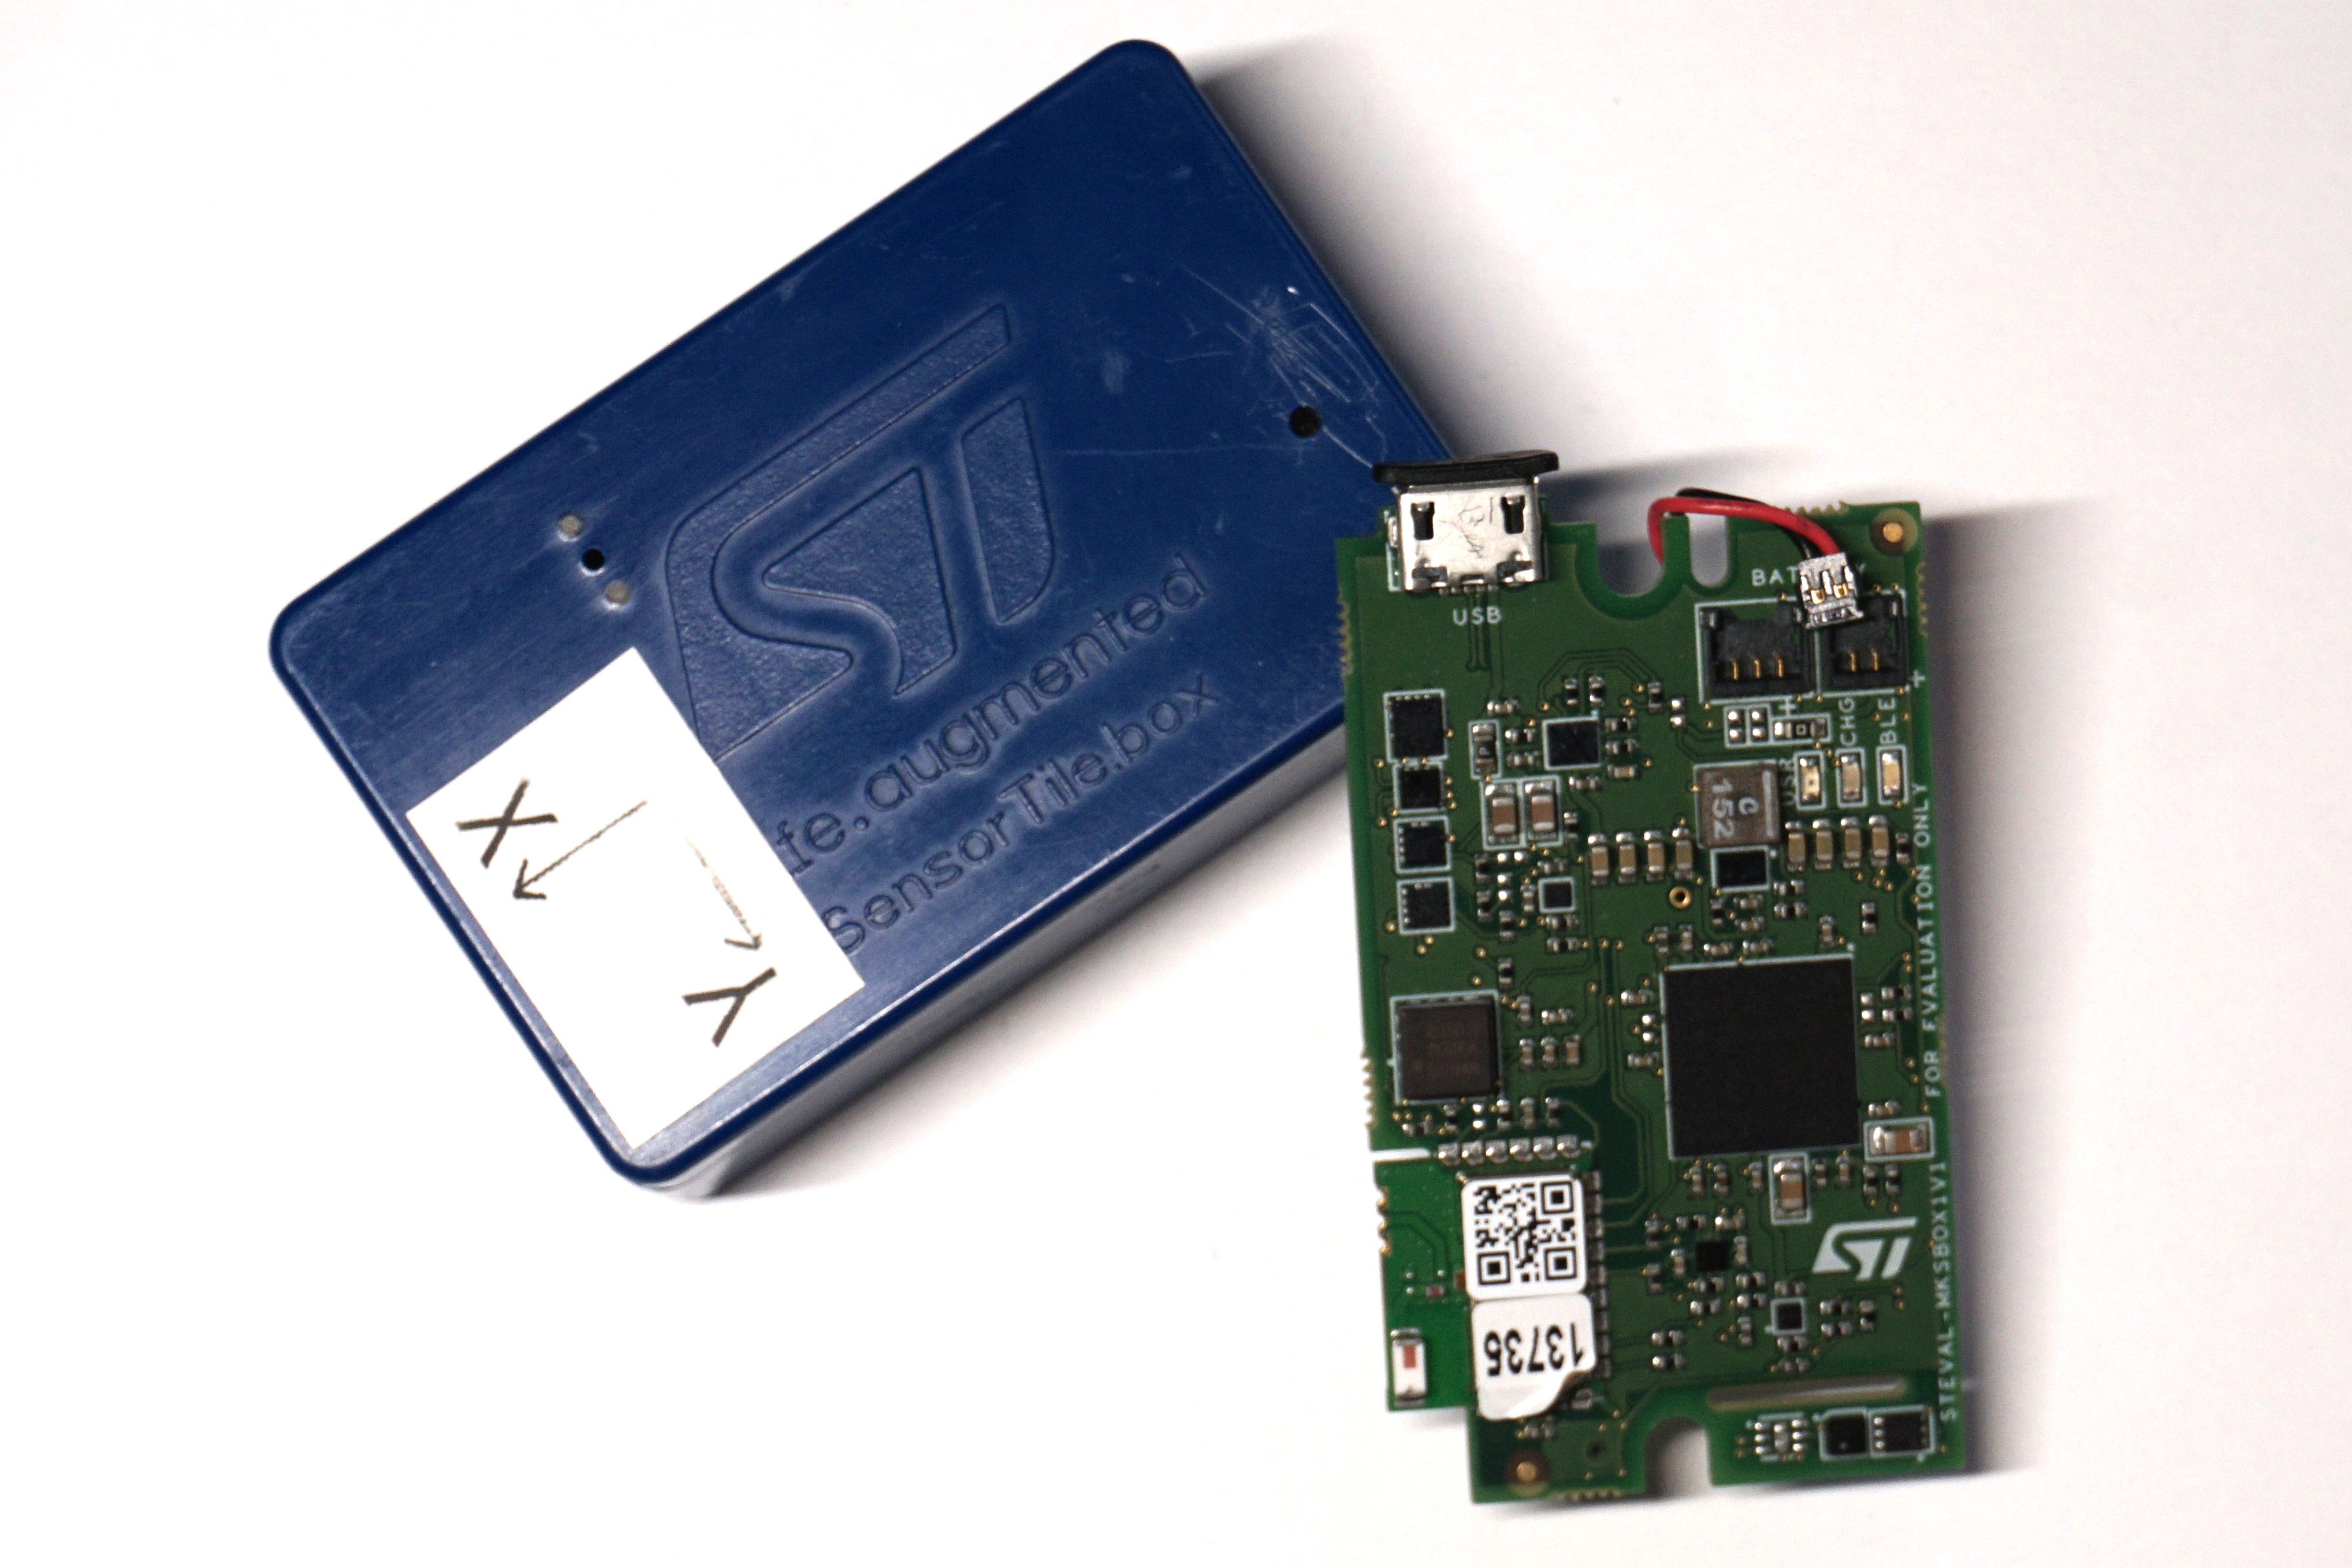
\includegraphics[width=0.75\textwidth]{chap2/figure/stbox.JPG}
        \caption{Image of the SensorTile.box, with the included case.}
        \label{fig:sensortilebox-image}
    \end{figure}

All the data coming from these sensors can be processed with the help of the embedded STM32L4R9 microcontroller, an ARM Cortex-M4 based processor containing DSP and FPU units. All the information can be then transmitted with the ST Bluetooth processor BlueNRG-M2, that supports Bluetooth Low Energy 5.2 specifications. 

The board comes with a preinstalled firmware that allows to read the sensor data via ST applications, or to log data inside an SD cart. The Android application also allows some firmware personalization, adding features like sensor fusion, audio FFT and so on. Anyway, there is no functionality that allows time synchronization of any type. 

If any developer wants to modify the firmware, it is possible to connect the peripheral to the computer and write a firmware using the STM32 development environment \cite{STM32dev}. Then, it is possible to write a firmware from scratch or to start from the available firmware examples (from GitHub or the ST website). The developer can then decide if they wants to keep compatibility with the ST applications or not, as they have total freedom on the board behaviour. 

ST offers an extensive set of Hardware Abstraction Layer (HAL) procedures, that makes it easy to develop firmware for the board and access functionality from both the sensors and the Bluetooth Low Energy stack.

Once the firmware is ready, the microcontroller can be flashed by means of ST solutions (ST-Link) or via an USB cable. The STM32CubeProgrammer \cite{STM32CubeProg} is the ST software that allows the programming. 

To conclude the overview, the kit contains a long-life USB-rechargeable battery and a case that provides water and dust resistance.  

\subsection{ST BlueTile}
The BlueTile from ST Microelectronics (STEVAL-BCN002V1B) is a development board containing a full set of MEMS sensors connected to a BlueNRG-2 SoC, that allows Bluetooth Low Energy connectivity. Here's the list of the embedded sensors:
\begin{itemize}
    \item  BALF-NRG-02D3: ultra-miniature balun and harmonic filter
    \item  LSM6DSO: iNEMO 6DoF inertial module, ultra-low power and high accuracy
    \item  LIS2MDL: magnetic sensor, digital output, 50 Gauss magnetic field dynamic range, ultra-low power, high performance, 3-axis magnetometer
    \item  VL53L1X: long range Time-of-Flight sensor based on ST FlightSense technology
    \item  MP34DT05TR-A: MEMS audio sensor omnidirectional digital microphone, 64~dB SNR, -26~dBFS sensitivity, top-port, 122.5~dBSPL AOP
    \item  LPS22HH: ultra-compact piezo-resistive absolute pressure sensor, 260-1260~hPa, digital output barometer, full-mold dust resistant, holed LGA package (HLGA)
    \item  HTS221: capacitive digital sensor for relative humidity and temperature 
\end{itemize}

      \begin{figure}[ht!]
        \centering
        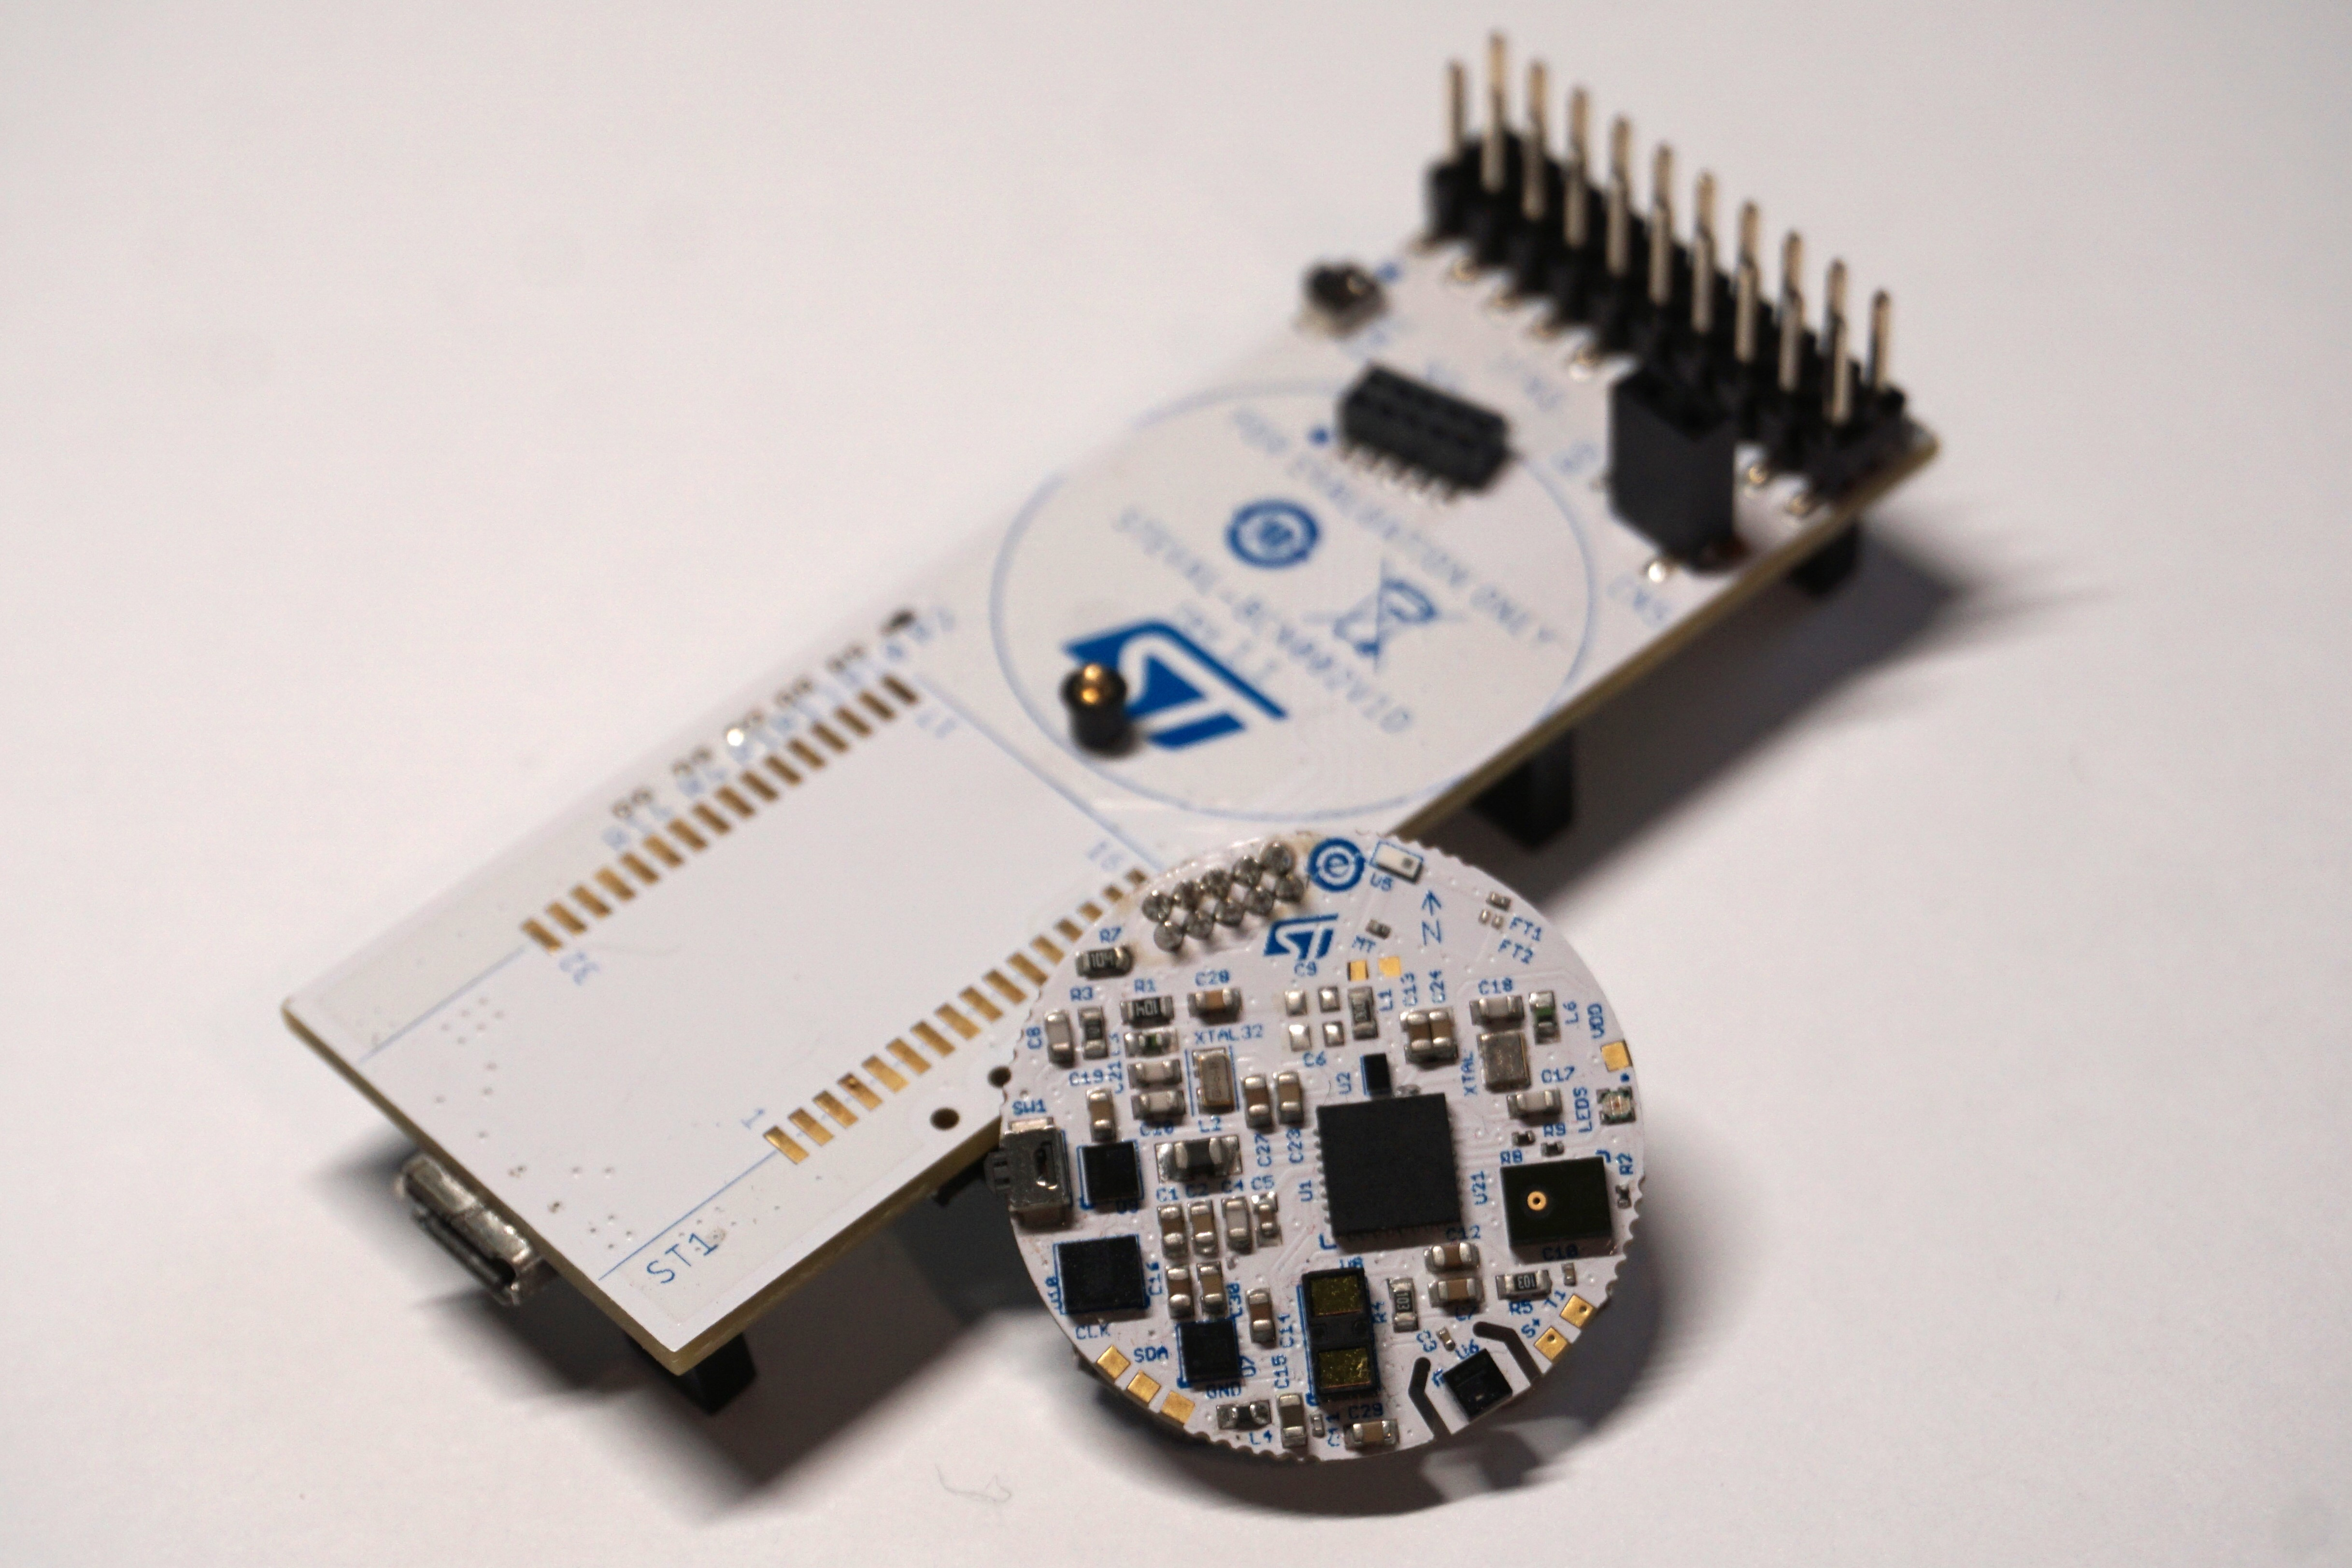
\includegraphics[width=0.75\textwidth]{chap2/figure/btile.JPG}
        \caption{Image of the BlueTile, with its programming board.}
        \label{fig:bluetile-image}
    \end{figure}

To perform elaboration and transmission of the resulting data, the embedded  SoC is a network processor for Bluetooth Low Energy that allows its own Cortex M0 core to be programmed by the user. In this way, no overhead is present, as one chip is enough to perform all the necessary operations for the board. Also in this case, ST released examples and low-level drivers, allowing the board to be programmed at high-level under both the BLE connectivity and sensor configuration aspects. 

The kit also contains a programming board, to which the small BlueTile can be connected: then, it can be programmed by means of a USB cable or a programming interface from ST (ST-link or ST NUCLEO  board), with the ST RF-Flasher software \cite{rfflasher}.

The board can be powered via an USB cable, when connected to its programming board, or via a CR2032 battery. ST advertises the sensors and the microcontroller to be battery-friendly, thanks to some hardware optimizations and their enhanced sleep states.

\subsection{MBIENTLAB MetaMotionS}
While ST solutions give a lot of freedom to the final user, making it easy for them to develop and personalize the firmware of the boards, MBIENTLAB solutions go in a different direction, offering devices with a complete set of sensors that are ready to use. In my case, I had at my disposal three MetaMotionS, containing the following set of sensors:
\begin{itemize}
    \item Bosch BMI270 6-Axis Accelerometer/Gyroscope
    \item Bosch BMM150 3-Axis Magnetometer
    \item Bosch BMP280 Digital Pressure Sensor
    \item Lite-On LTR-329ALS-01 Ambient Light Sensor
    \item I/O analog and digital pins are present for expansion purposes.
\end{itemize}

      \begin{figure}[ht!]
        \centering
        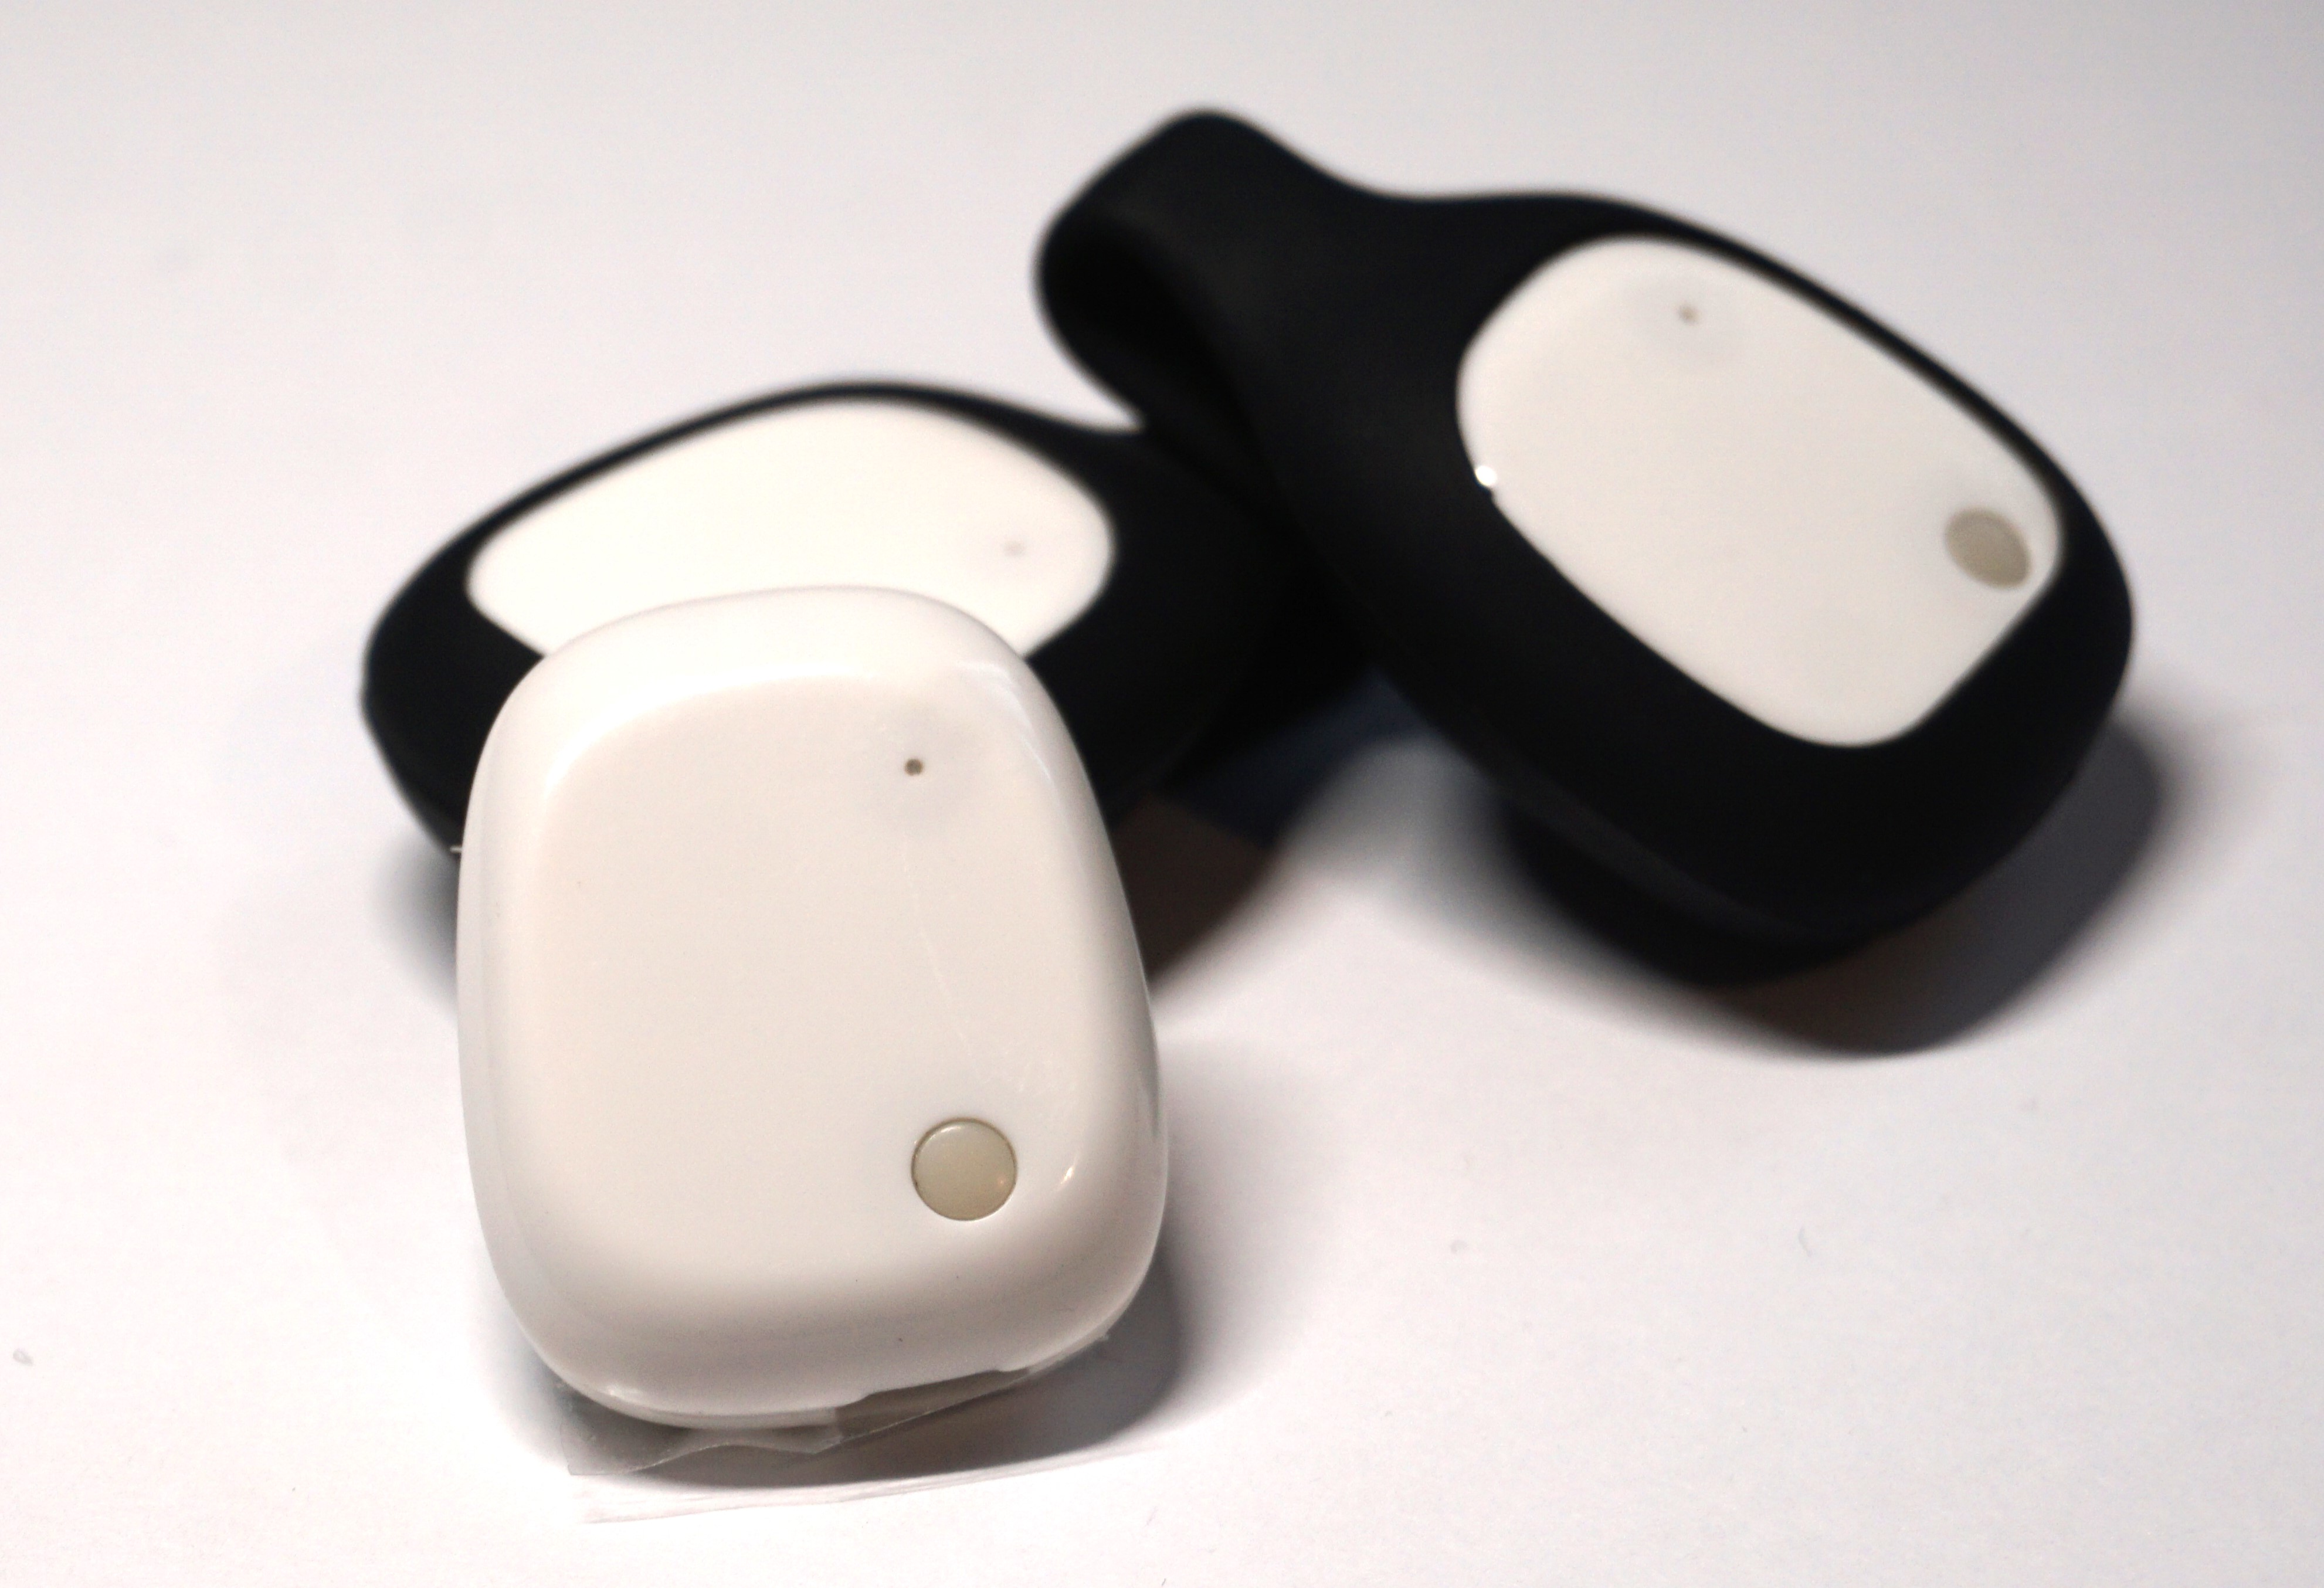
\includegraphics[width=0.75\textwidth]{chap2/figure/mms.JPG}
        \caption{Image of the MetaMotionS devices, with and without the clip accessory.}
        \label{fig:mms-image}
    \end{figure}

All the sensors are connected to a Nordic Semiconductor nRF52840 BLE SoC, which is the network chip whose Cortex-M4 processor allows heavy data elaboration (including 9-axis sensor fusion algorithms). The sensors information can be transmitted via both Bluetooth Low Energy protocols and USB. The provided firmware is closed source and can't be modified. 

The device comes in a water-resistant case enclosure that can be put in (optional) wearable accessories, like clips and wristbands and it contains a USB-rechargeable battery. The mobile application available, MetaBase \cite{metabase}, allows a complete configuration of the sensors, that can be turned on/off and configured in their data rate and precision. Once everything is set-up, the application can start the data recording, that can be streamed directly on the mobile device or saved in the 512~MB internal  memory, to be downloaded later. 

The most interesting part of these products are the open-source APIs that are available \cite{metawearapi}, making the devices easily configurable and usable from any BLE-supported computer or smartpoone with a reduced number of lines of code. In particular, they are available for Android (Java), iOS (Swift), Linux (Javascript, Python), Windows (Python) and already include all the necessary libraries and procedures for Bluetooth connectivity. A C++ library is also available, to be adapted to other operating systems and their Bluetooth stacks. The APIs are well-documented on their website, while their GitHub profile contain a lot of examples ready to be personalized to the user needs. 

To conclude this overview, it is important to add that these boards firmwares already contain a sort of synchronization mechanism. All the data coming from them is precisely timestamped with a UNIX Epoch time, in particular with a millisecond resolution. 



% There are a wide variety of approximate solvers for NP-Optimization problems. The ones presented in this chapter are classified as \textit{metaheuristics}, that is, they are higher-level algorithms that implement mechanisms to choose between various strategies to explore the solution space. As such, the fundamental difference between them is the implementation of the "artificial intelligence" driving this choice; the inspiration behind this implementation has often come from observations in the fields of biology and physics, with algorithm designers trying to reproduce the innate efficiency of natural phenomena. Metaheuristic methods make extensive use of stochastic optimization for an effective exploration of the search space, and require very few assumptions \textit{a priori} about the problem to be solved, therefore they are applicable to a wide range of problems with a few adaptations.
%\begin{itemize}
%\newpage

%\endinput